\section{Results}
\textbf{Note}: The phrase indel refers to gene insertion/deletion events. It is impossible to tell between two \ac{otu}s if a gene was deleted from one or inserted in the other.
Thus such discrepancies are referred to as indels, inferred to be the result of \ac{hgt} between the two \ac{otu}s.
%example network
%Fig
\FloatBarrier
\begin{figure}[htb!]
    \makebox[\textwidth][c]{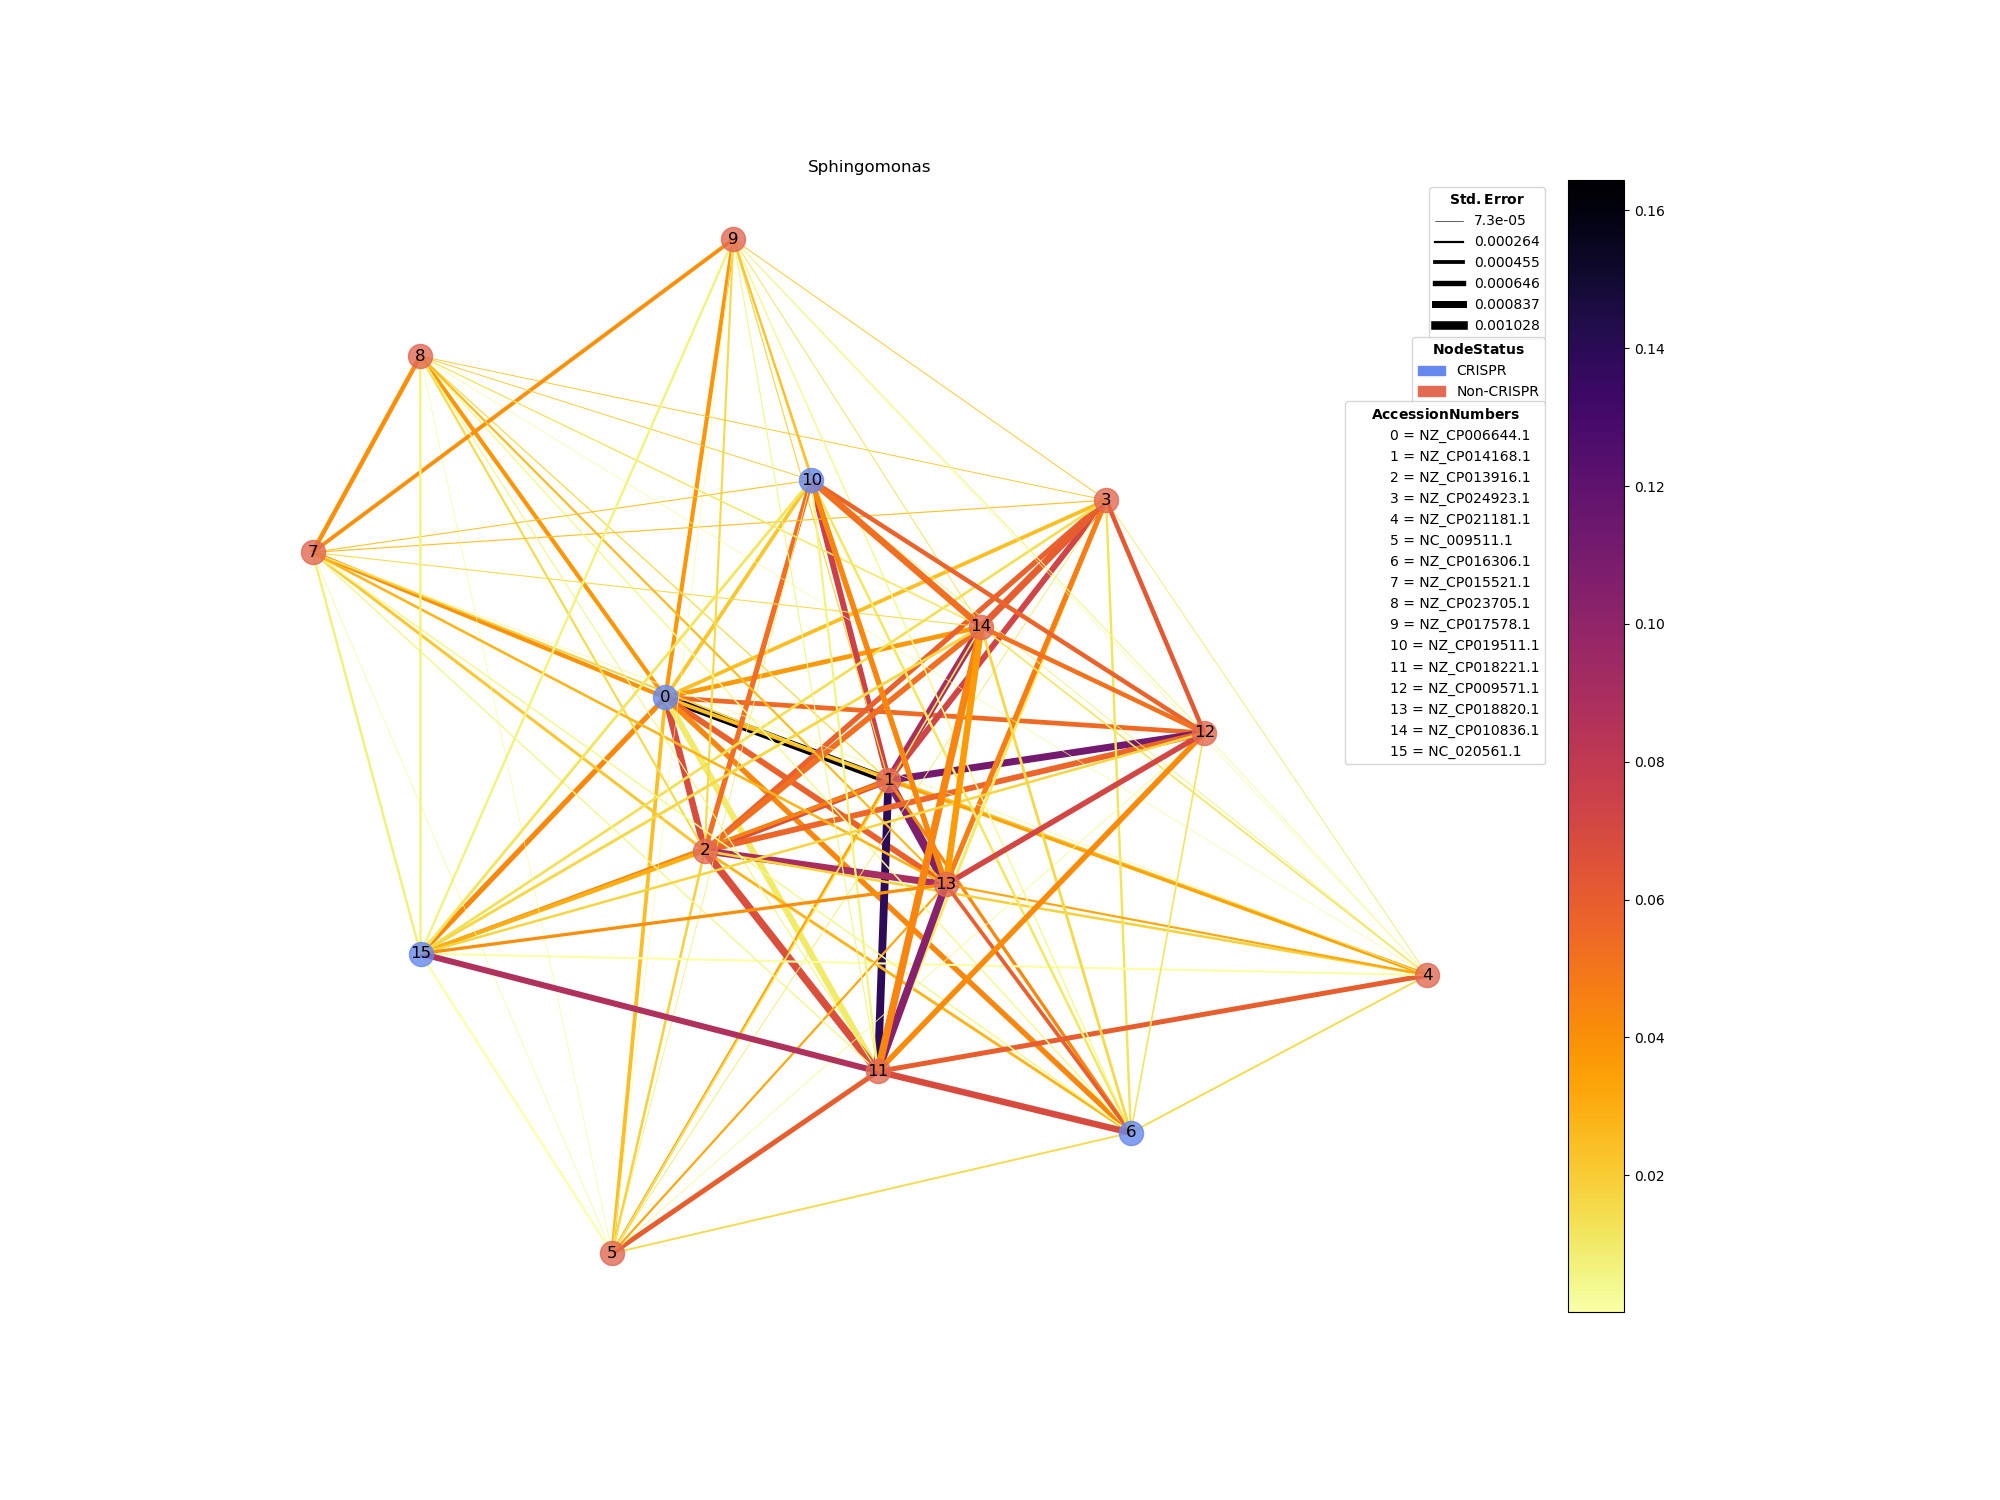
\includegraphics[width=1.3\linewidth]{network.png}}
    \caption{Example of a \ac{hgt} network produced by HiDe. This network is a ``consensus'' over 1000 bootstap replicate networks, produced from sampling gene trees. Each bootstrap replicate was produced from 50 randomly sampled gene trees froma a total of 376 individual gene trees. Blue nodes were cassified as having a \ac{crsp} system, red nodes were not. Color represents the fraction of genes examined that were transfered along that edge. Width represents the standard error of the edge value over the 1000 bootstraps. (Note the maximum value for an edge is 1.00, meaning all examined genes were transfered along that edge)}
    \label{net}
\end{figure}
\FloatBarrier
%Desc
In figure \ref{net} it appears that several nodes have weak connections with most other nodes but strong connections with a few nodes.
Further both \ac{crsp} and non-\ac{crsp} nodes both show distributions of strong and weak connections with other \ac{crsp} and non-\ac{crsp} nodes both.
Also the standard error of each edge appears proportional to it's weight.
This is likely due to the sampling, as if more genes were transferred along an edge, the more likely some of those genes were left out of any individual bootstrap sample, as the size of each bootstrap sample was $\frac{50}{376}$ of the total number of gene trees.
%degree bar
\FloatBarrier
\begin{figure}[htb!]
    \makebox[\textwidth][c]{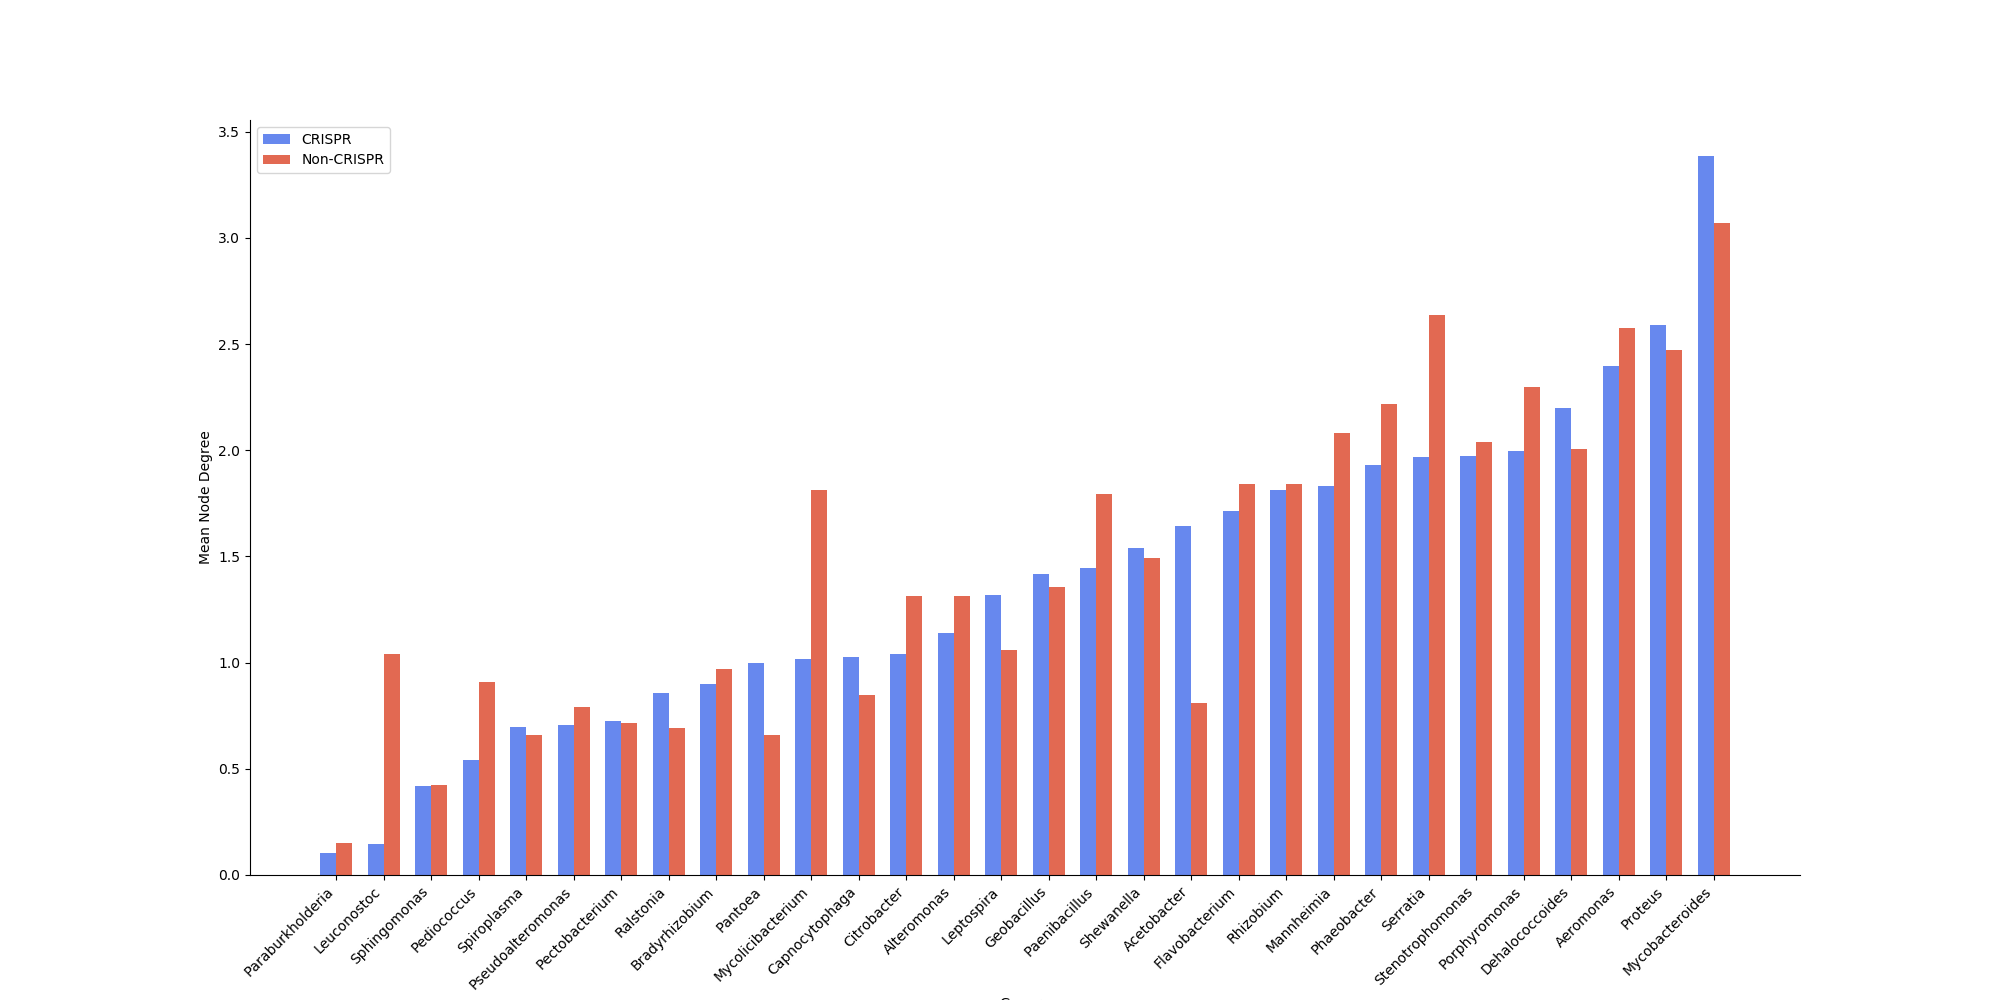
\includegraphics[width=1.3\linewidth]{c_nc_deg_bar.png}}
    \caption{Mean node degree for either all \ac{crsp} or Non-\ac{crsp} nodes across all 1000 bootstrap replicates for each genus. There were 30 genera used.}
    \label{db}
\end{figure}
\FloatBarrier
%indel bar
%Fig
\FloatBarrier
\begin{figure}[htb!]
    \makebox[\textwidth][c]{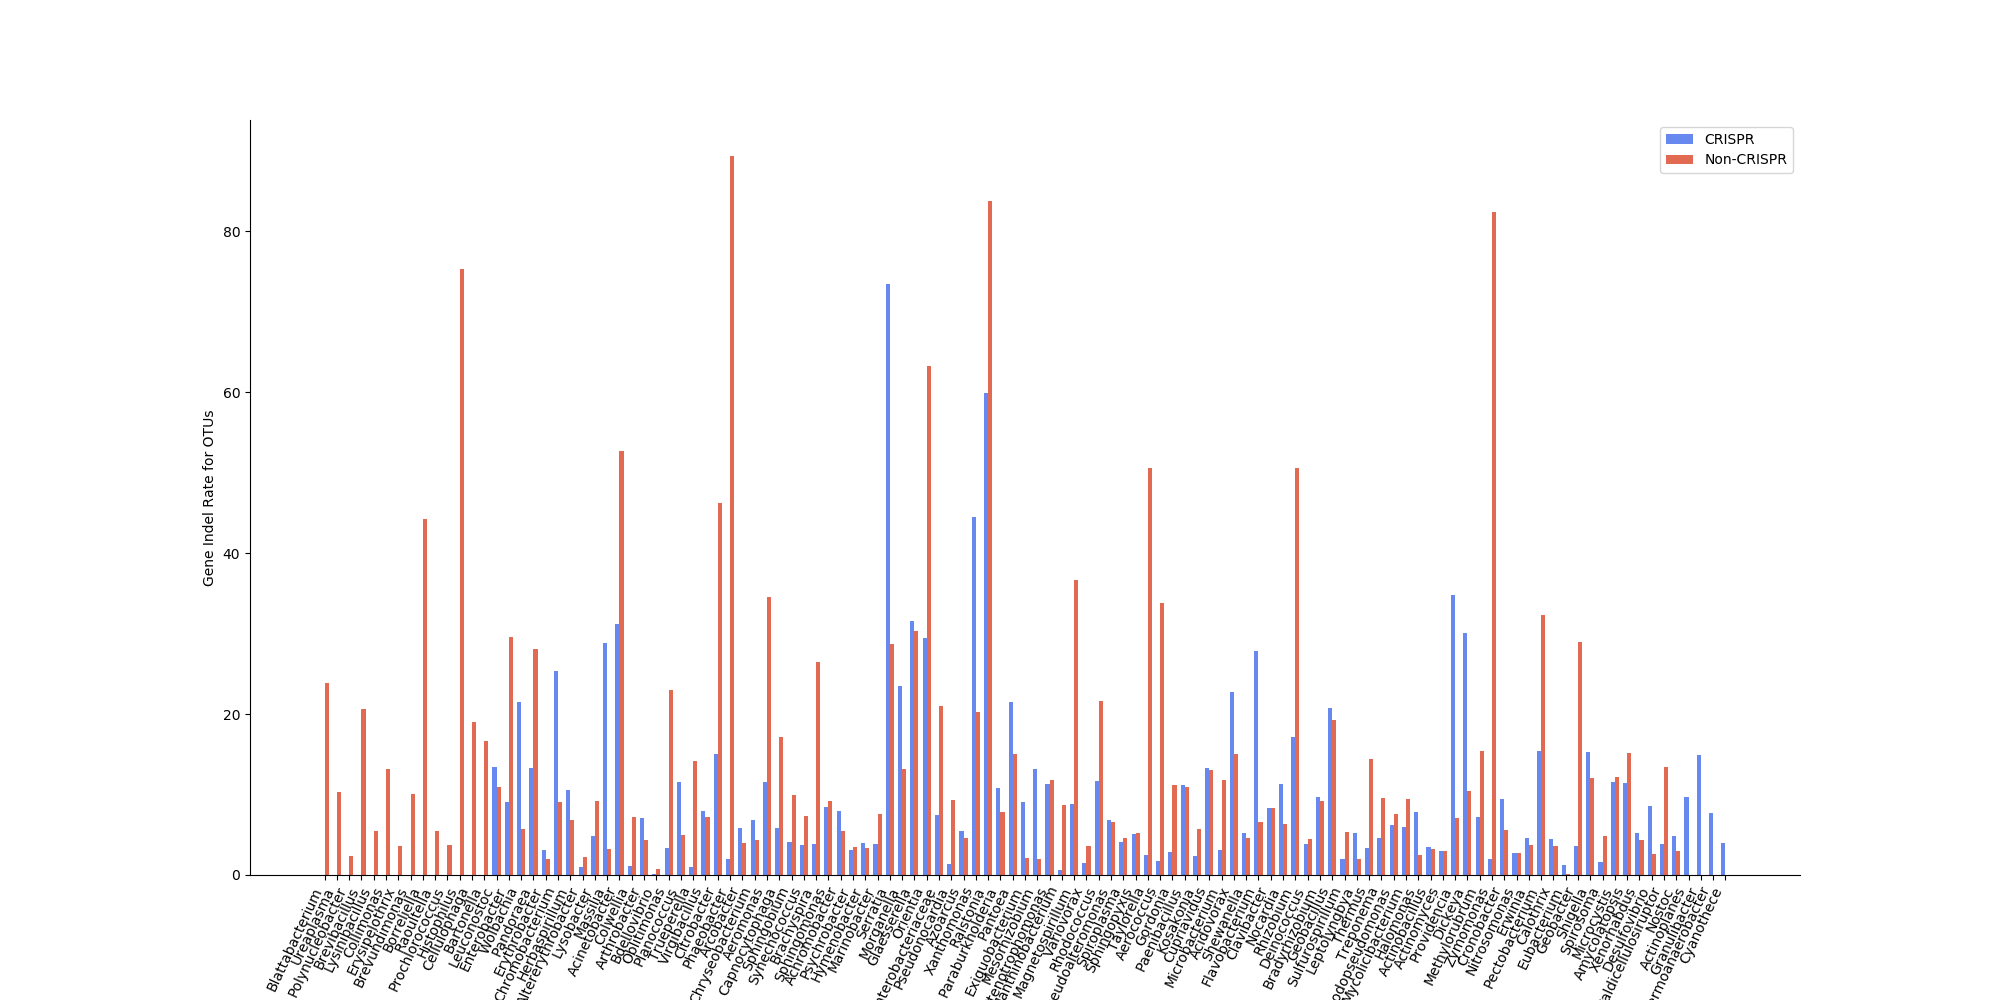
\includegraphics[width=1.3\linewidth]{c_nc_indel_bar.png}}
    \caption{Markopholo estimate of gene indel rates for the partitions of \ac{crsp} and Non-\ac{crsp} \ac{otu}s for each genus. Rate is indel events per base pair substitution. There were 140 genera used.}
    \label{ib}
\end{figure}
\FloatBarrier
%Desc
The mean node degree is much more similar between the \ac{crsp} and non-\ac{crsp} than the indel rate estimates (figures \ref{db},\ref{ib}).
Both show significant variability for the non-\ac{crsp} nodes across genera, but the indel rates estimates for the \ac{crsp} nodes are much less variable and generally smaller by comparison.
Despite this there are clear exceptions where the indel rate is estimated to be much larger for \ac{crsp} \ac{otu}s than non-\ac{crsp} \ac{otu}s, specifically of Rhizobium, Acetobacter, Pediococcus and Moraxella.
%indel scatter
%Fig
\FloatBarrier
\begin{figure}[htb!]
    \makebox[\textwidth][c]{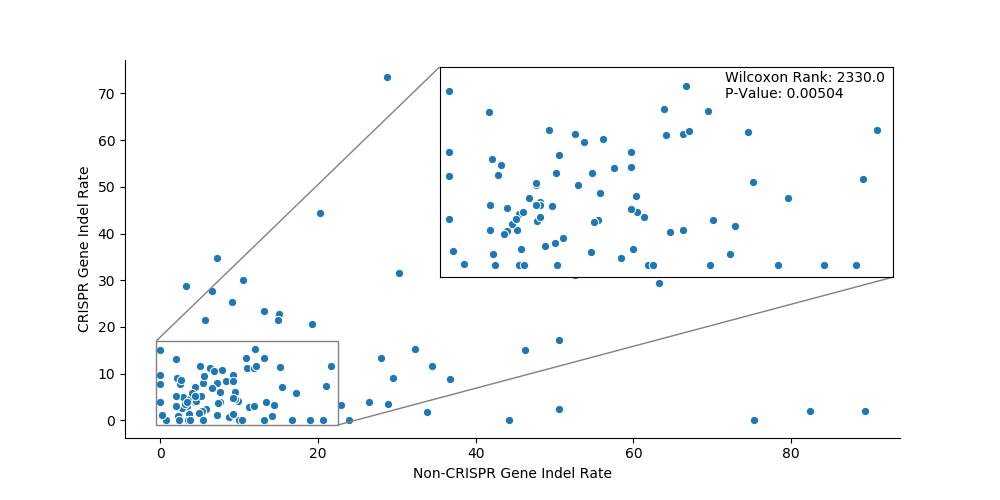
\includegraphics[width=1.3\linewidth]{c_nc_rate_scatter.png}}
    \caption{Markopholo estimate of gene indel rates for the partitions of \ac{crsp} and Non-\ac{crsp} \ac{otu}s for each genus. Rate is indel events per base pair substitution. Each point represents a genus. There were 140 genera used.}
    \label{is}
\end{figure}
\FloatBarrier
%Desc
Figure \ref{is} further demonstrates these points, that \ac{crsp} indel rates are smaller and less varied that the and non-\ac{crsp}.
This difference is quantified by the Wilcoxon signed rank test statistic of $191,0$ and a corresponding p-value $0.02596$.
%crispr frac vs rate difference
%Fig
\FloatBarrier
\begin{figure}[htb!]
    \makebox[\textwidth][c]{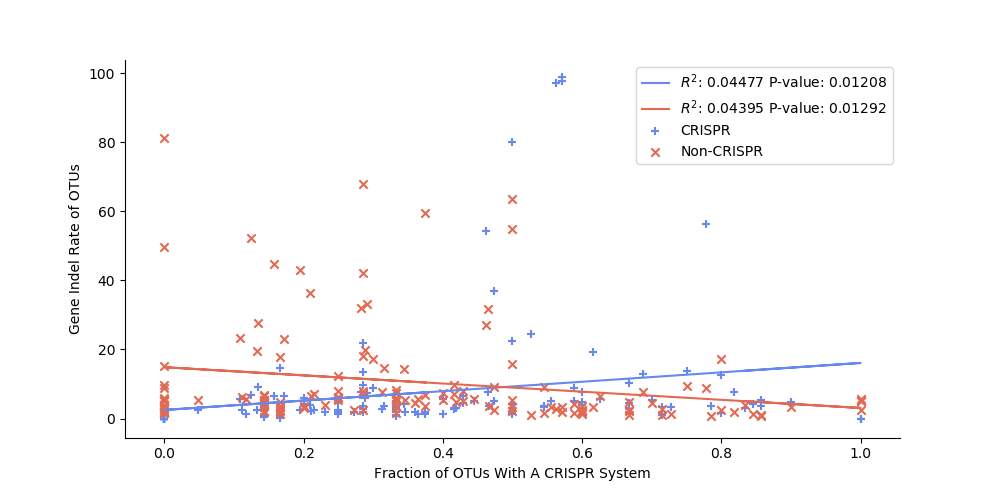
\includegraphics[width=1.3\linewidth]{cfrac_cncRateDiff_scattter.png}}
    \caption{Markopholo estimate of gene indel rates for the partitions of \ac{crsp} and Non-\ac{crsp} \ac{otu}s for each genus against the fraction of all \ac{otu}s in that genus that are annotated as having a \ac{crsp} system. $R^2$ values are for linear regression lines fit to the \ac{crsp} and non-\ac{crsp} estimates. Rate is indel events per base pair substitution. Each point represents a genus. There were 140 genera used.}
    \label{cfrd}
\end{figure}
\FloatBarrier
%Desc
Figure \ref{cfrd} show that as the fraction of all \ac{otu}s in a genus with a \ac{crsp} system increases, the gene indel rates appear to decrease for non-\ac{crsp} \ac{otu}s remains mostly stagnant for \ac{crsp} \ac{otu}s.
The $R^2$ values in figure \ref{cfrd} are fairly small, implying a poor fit of a linear relationship to the data, but the p-values are significant, implying that some relationship does exist.
%Cluster C NC
%Fig
\FloatBarrier
\begin{figure}[htb!]
    \makebox[\textwidth][c]{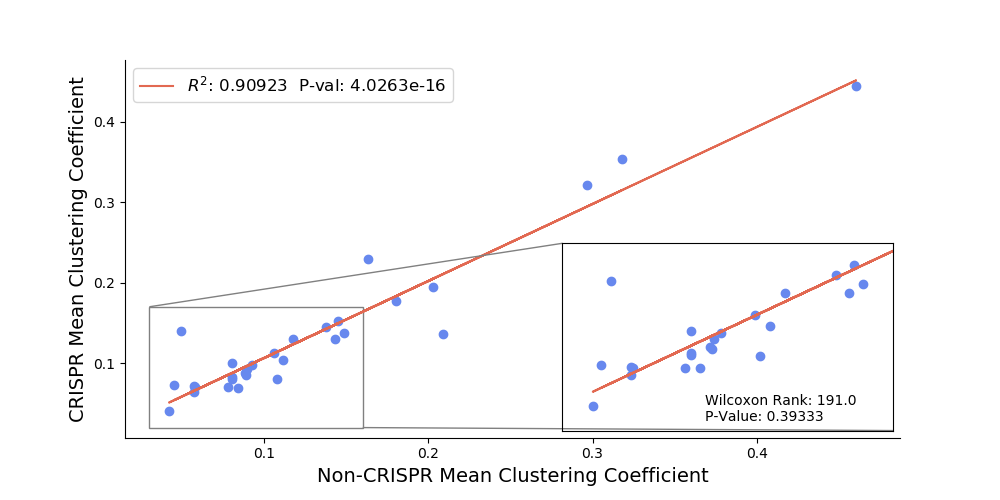
\includegraphics[width=1.3\linewidth]{c_nc_clust_scatter.png}}
    \caption{Mean over 1000 bootstraps of the clutering coefficients of the \ac{crsp} \ac{otu}s for each genus against the non-\ac{crsp} means over the 1000 bootstraps. $R^2$ value is for the linear regression fit to the \ac{crsp} and non-\ac{crsp} estimates. There were 140 genera used.}
    \label{ccnc}
\end{figure}
\FloatBarrier
%Desc
Figure \ref{ccnc} show the mean clustering coefficient over 1000 bootstraps for each genus for all \ac{crsp} and non-\ac{crsp} \ac{otu}s.
There appears to be a clear linear relationship between the mean clustering coefficients of \ac{crsp} and non-\ac{crsp} \ac{otu}s.
Clustering is also generally small in magnitude, with most of the data in the range of $0.0$ to $0.2$ (the maximum value is $1.0$).
%modularity
%Fig
\FloatBarrier
\begin{figure}[htb!]
    \makebox[\textwidth][c]{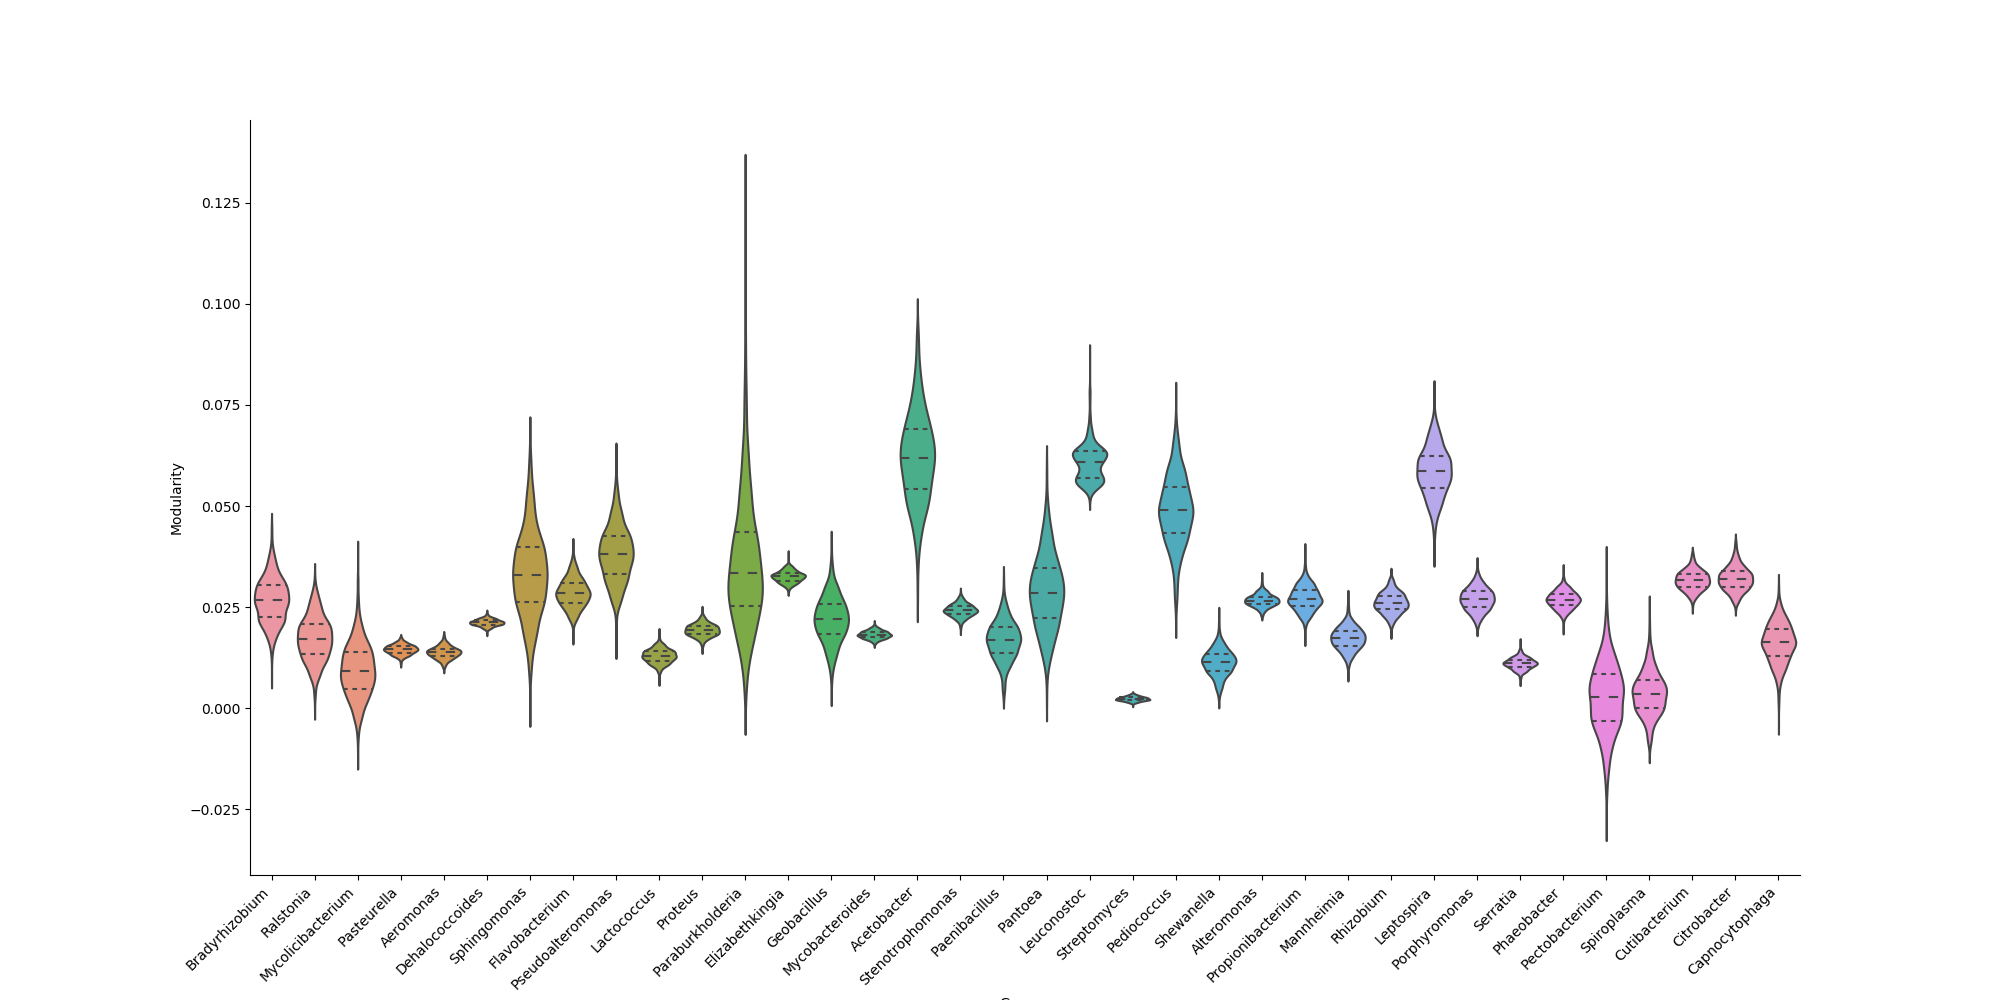
\includegraphics[width=1.3\linewidth]{mod_violin.png}}
    \caption{Distribution of network modularity over 1000 bootstrap repliactes for each genus. Plot is of the kernel density estimated from the observed values, with witdh proportional to the number of data points. Lines inside each distribution represent quartiles.}
    \label{mod}
\end{figure}
\FloatBarrier
%Desc
Figure \ref{mod} shows that the distribution of network modularity is centered near $0$ for most networks, implying a lack of modularity between \ac{crsp} and non-\ac{crsp} \ac{otu}s.
However the variability in the shape of each distribution, ranging from very narrow to very wide, with some being bimodal, should be noted.
%Assortativity
%Fig
\FloatBarrier
\begin{figure}[htb!]
    \makebox[\textwidth][c]{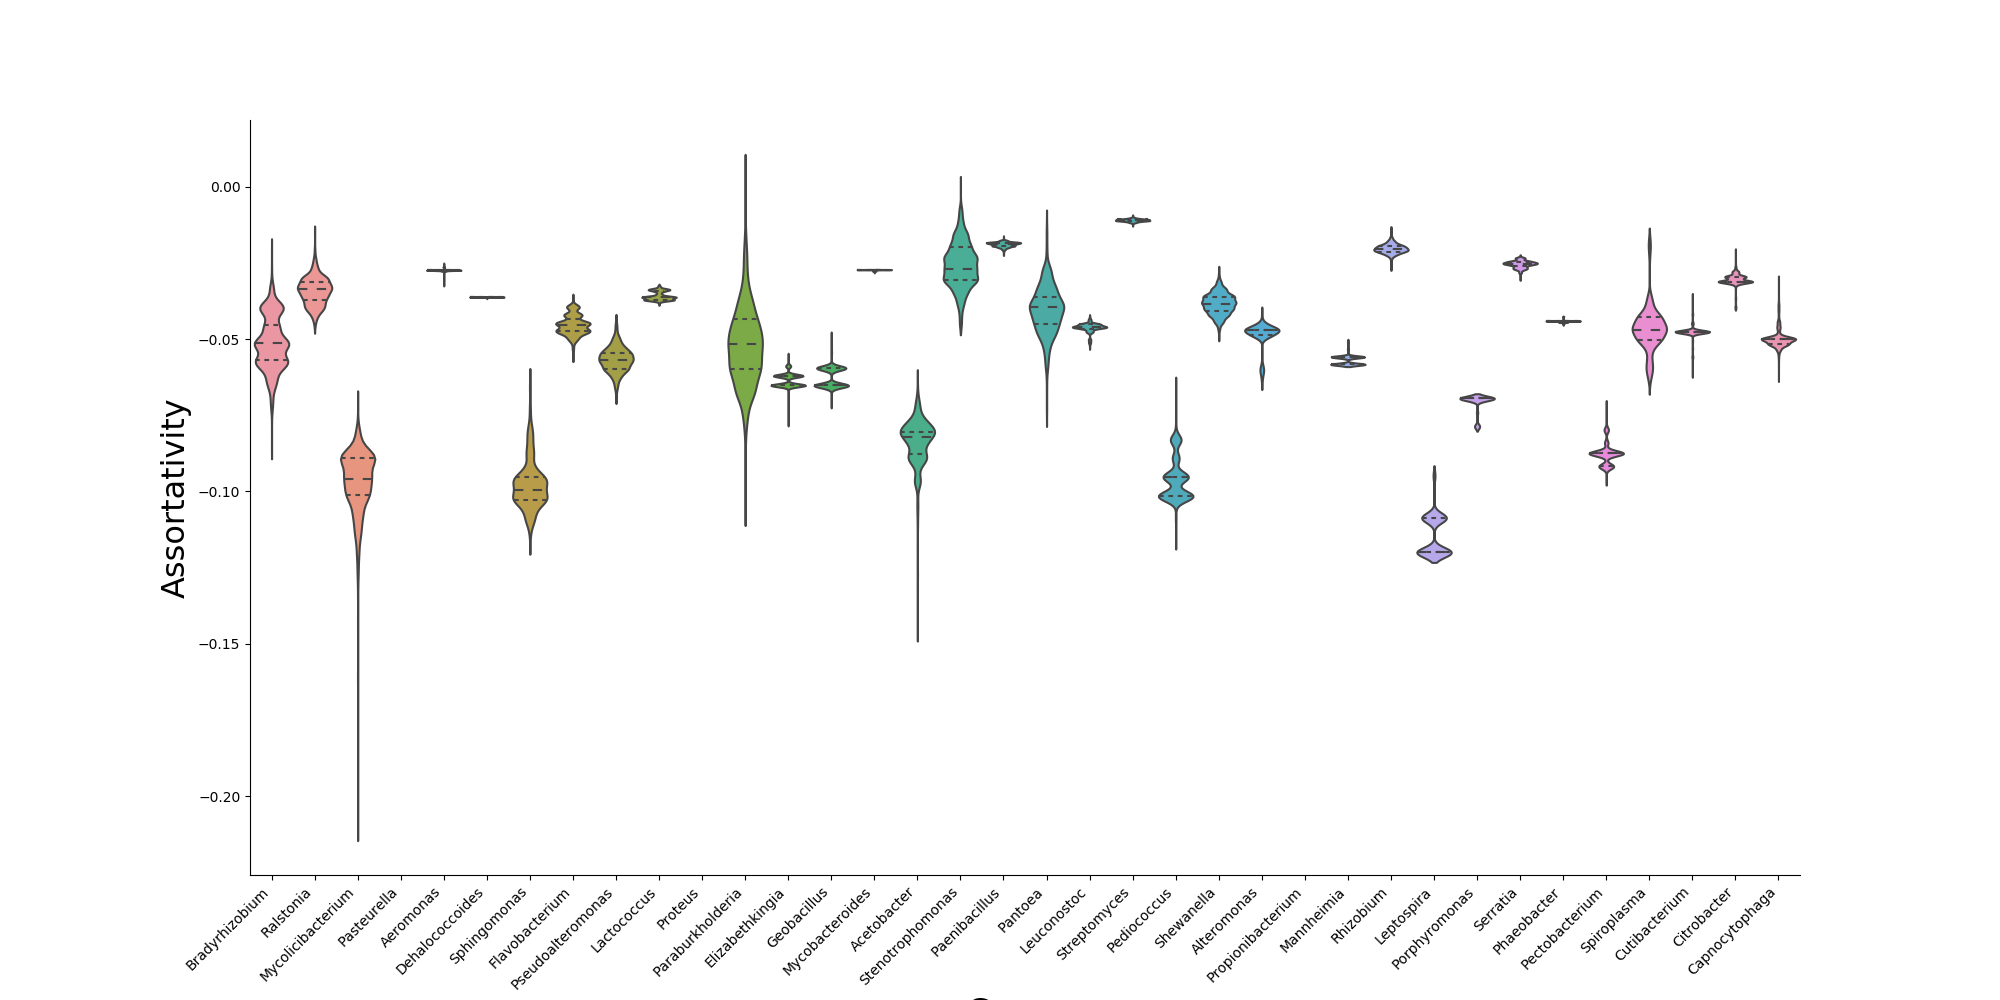
\includegraphics[width=1.3\linewidth]{asst_violin.png}}
    \caption{Distribution of network assortativity by \ac{crsp} status (either \ac{crsp} or non-\ac{crsp}) over 1000 bootstrap repliactes for each genus. Plot is of the kernel density estimated from the observed values, with witdh proportional to the number of data points. Lines inside each distribution represent quartiles.}
    \label{asst}
\end{figure}
\FloatBarrier
%Desc
Figure \ref{asst} shows that the distribution of network assortativity is centered near $-0.05$ for most networks, implying a lack of assortativity between \ac{crsp} and non-\ac{crsp} \ac{otu}s.
The variability in the shape of each distribution is much more pronounced than with modularity, with many distributions having several undulations or very sharp contrasts between different peaks or completely smooth and centered around the mean.
This variability may be due to the variation in the fraction of \ac{otu}s with a \ac{crsp} system.
Some genera may only have one or two \ac{otu}s with a \ac{crsp} system, thus limiting the range of values that assortativity can take on, due to how it is defined.
%%pairplot
%\FloatBarrier
%\begin{figure}[htb!]
%    \makebox[\textwidth][c]{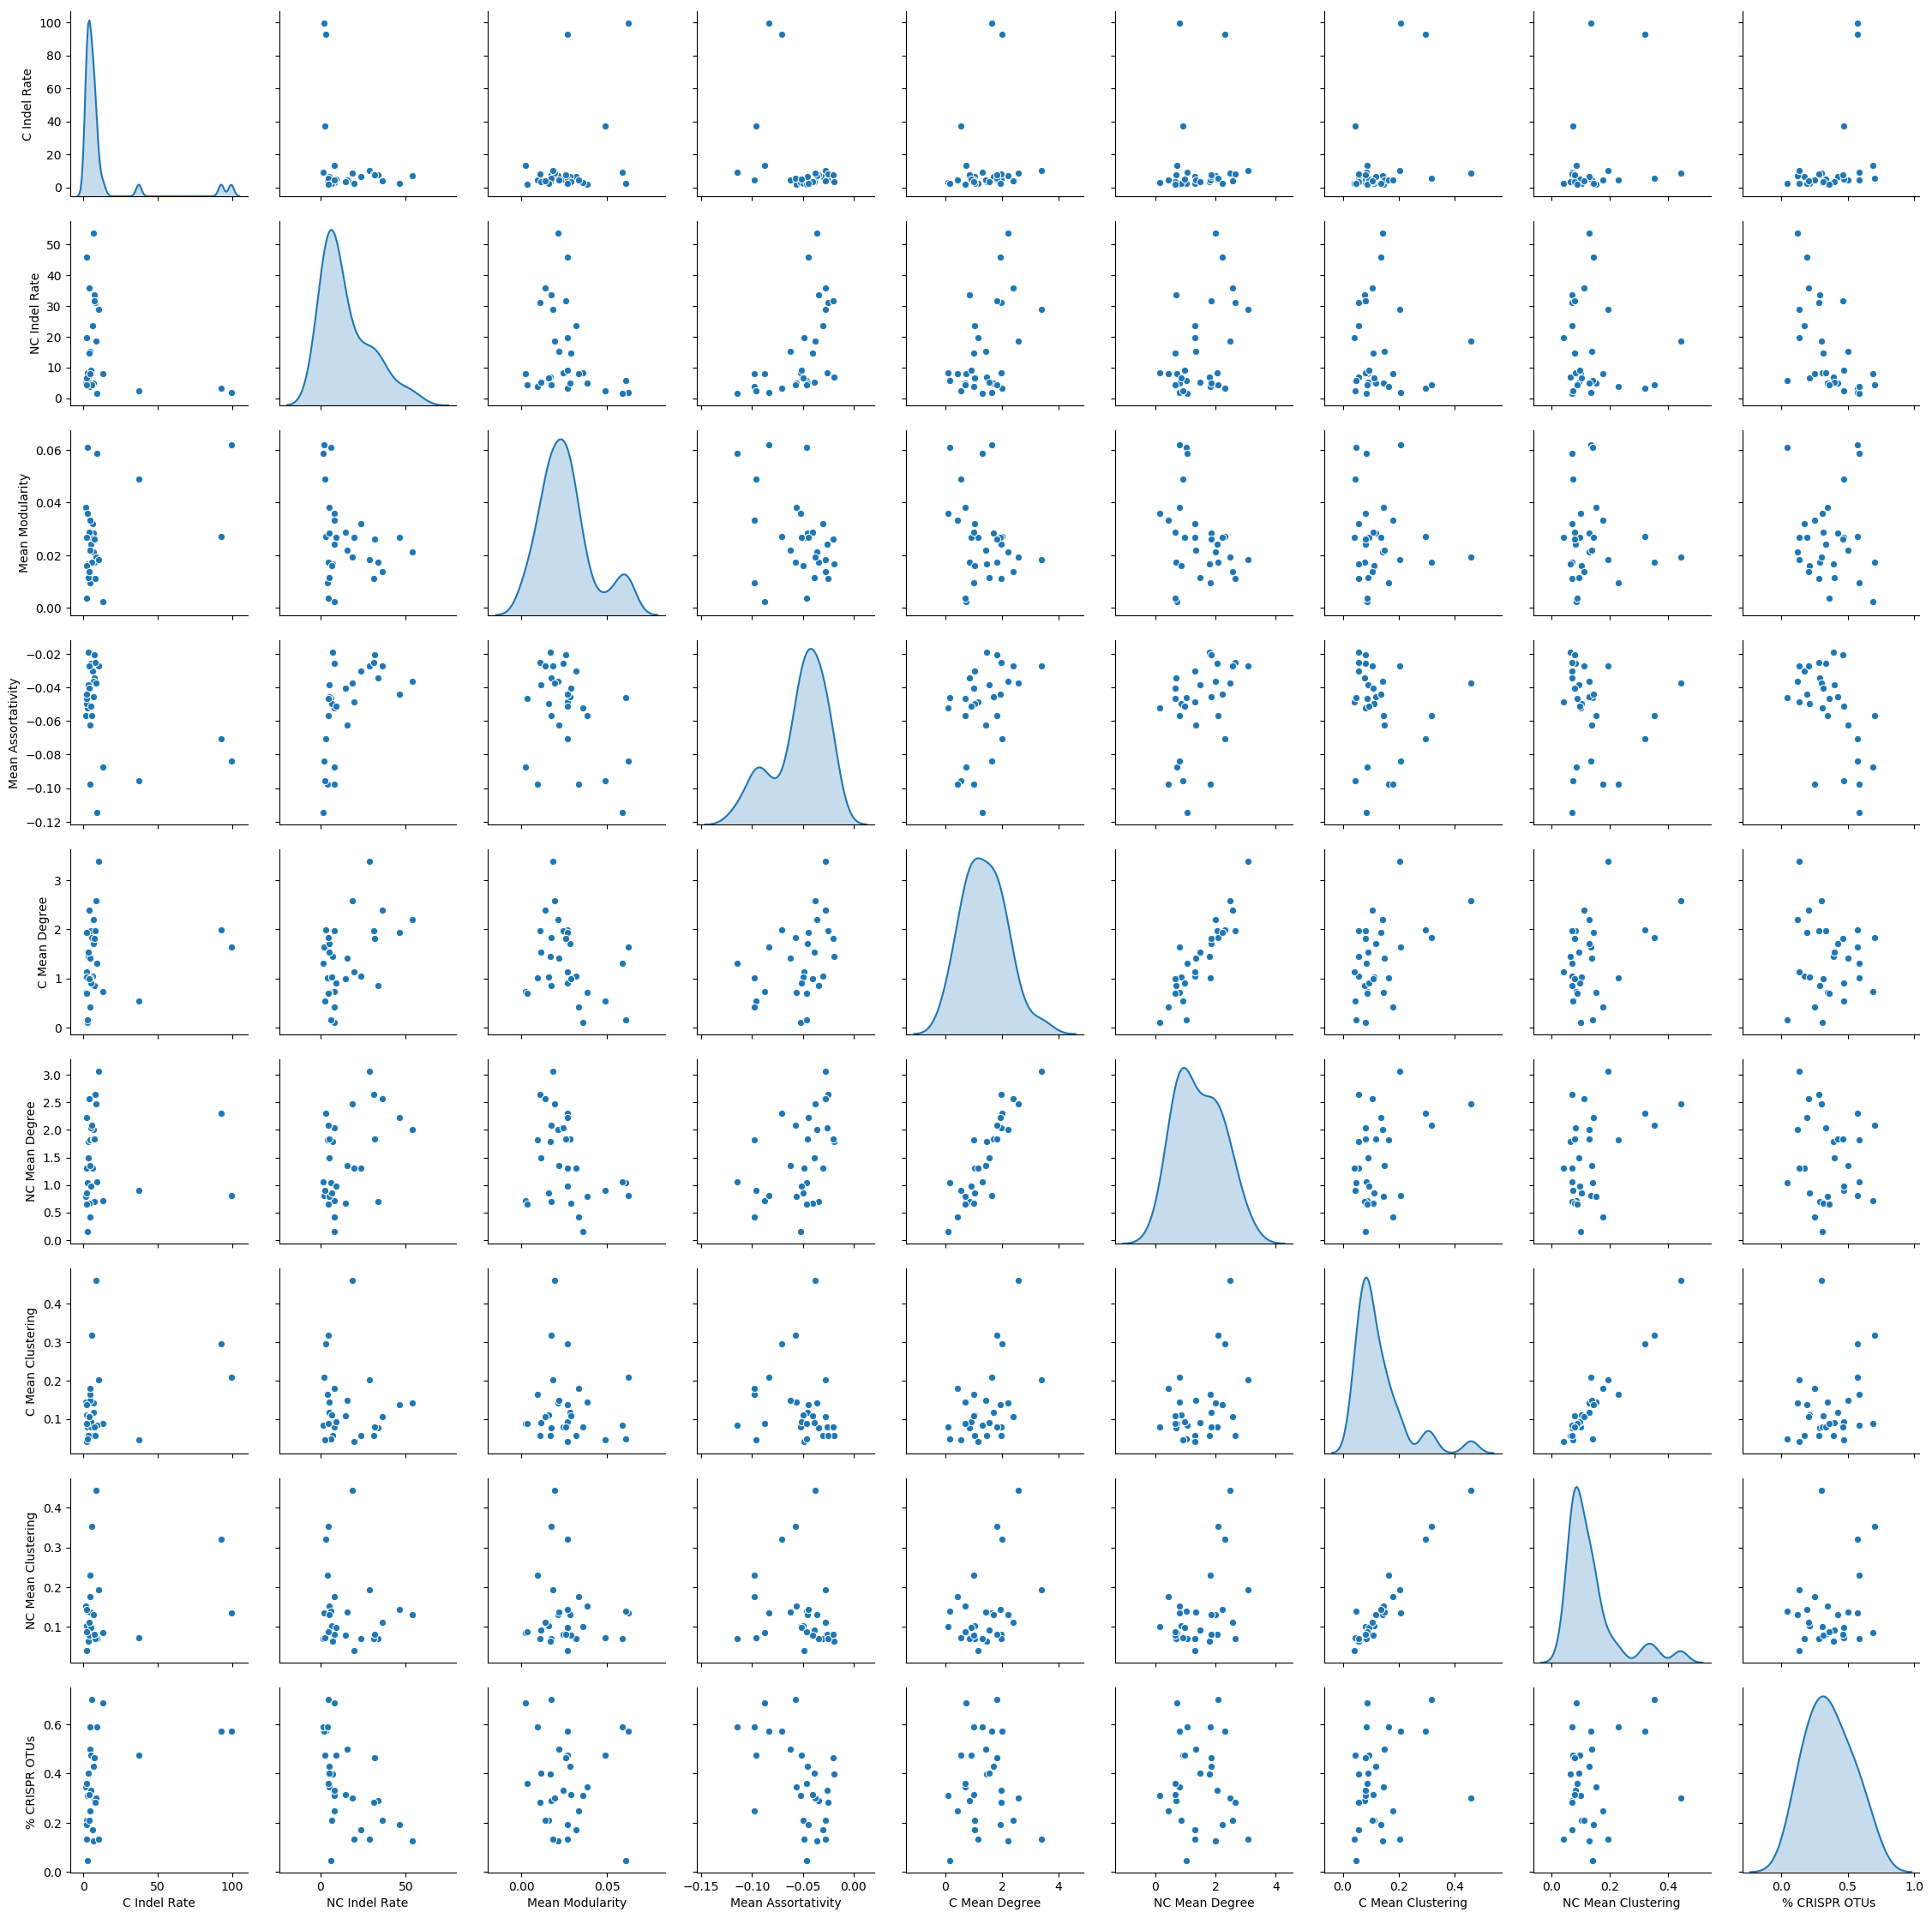
\includegraphics[width=1.3\linewidth]{pairplot.png}}
%\end{figure}
%\FloatBarrier
